\documentclass[sigconf,screen,nonacm]{acmart}
\usepackage{booktabs,tabularx,array,amsmath,listings}
\usepackage[nospread,noshrink]{flushend}
\makeatletter
\@ACM@balancefalse
\makeatother
\raggedbottom
\definecolor{GSBlue}{HTML}{0072B2}
\definecolor{GSGreen}{HTML}{00876C}
\definecolor{GSInk}{HTML}{1D2939}
\settopmatter{printacmref=false,printfolios=true}
\renewcommand\footnotetextcopyrightpermission[1]{}
\setcopyright{none}
\acmDOI{}\acmISBN{}\acmConference{}{}{}\acmYear{2026}
\hypersetup{colorlinks=true,linkcolor=GSBlue,citecolor=GSBlue,urlcolor=GSBlue}
\setlength{\emergencystretch}{1.5em}
\newcolumntype{Y}{>{\raggedright\arraybackslash}X}
\newcommand{\code}[1]{\texttt{#1}}
\lstset{basicstyle=\ttfamily\scriptsize,breaklines=true,columns=fullflexible,showstringspaces=false,frame=single,rulecolor=\color{black!15},backgroundcolor=\color{black!2},xleftmargin=1mm,xrightmargin=1mm}
\graphicspath{{figures/}}
\title[GazeSync: Screen Interaction and Multi-Source Eye Tracking]{GazeSync: Reproducible Synchronization of Screen Interaction and Multi-Source Eye Tracking}
\settopmatter{authorsperrow=4}
\author{Yaxiong Lei}
\authornote{Working author list for review. Implementation report draft, 15 October 2026; not an accepted conference paper. Implementation arXiv submission pending.}
\affiliation{\institution{University of St Andrews and University of Essex}\city{St Andrews / Colchester}\country{United Kingdom}}
\author{Rishab Talwar}
\affiliation{\institution{University of St Andrews}\city{St Andrews}\country{United Kingdom}}
\author{Shijing He}
\affiliation{\institution{King's College London}\city{London}\country{United Kingdom}}
\author{Xinya Gong}
\affiliation{\institution{University of St Andrews}\city{St Andrews}\country{United Kingdom}}
\author{Yuheng Wang}
\affiliation{\institution{University of St Andrews}\city{St Andrews}\country{United Kingdom}}
\author{Xudong Cai}
\affiliation{\institution{King's College London}\city{London}\country{United Kingdom}}
\author{Zhongliang Guo}
\affiliation{\institution{University of St Andrews}\city{St Andrews}\country{United Kingdom}}
\author{Juan Ye}
\affiliation{\institution{University of St Andrews}\city{St Andrews}\country{United Kingdom}}
\authorsaddresses{}
\renewcommand{\shortauthors}{Lei et al.}
\begin{document}
\begin{abstract}
A gaze sample and a zoom event can arrive together even though they describe
different screen states. Recovering attention on manipulated content therefore
requires explicit temporal and spatial provenance. We extend GazeSync into a
standalone Python and TypeScript framework for desktop and mobile interaction,
2D points of gaze, 3D eye-origin rays, and independent monocular or binocular
streams. The framework separates capture, input, presentation and receipt time;
joins each observation to a surface-specific presentation history; and preserves
uncertainty, eye identity, geometry and missing data in a replayable record.
SDK-independent adapters normalize model and tracker records without assuming
equal acquisition rates or manufacturing confidence. A reproducible synthetic
matrix spans 78 configurations and 107,070 observations, including 30--240\,Hz
displays, 30--2,000\,Hz gaze and nine viewport sizes. Both implementations select
the reference capture frame in every case; maximum cross-language viewport
disagreement is $4.55\times10^{-13}$ logical pixels. These are numerical
consistency results, not physical tracking-accuracy estimates. We provide an
inspectable synchronization contract, diagnostic guidance, simulation fixtures
and isolated distribution tooling, and identify the device measurements needed
before making end-to-end accuracy claims.
\end{abstract}
\keywords{eye tracking, temporal synchronization, pan and zoom, binocular gaze, reproducibility, research software}
\begin{teaserfigure}
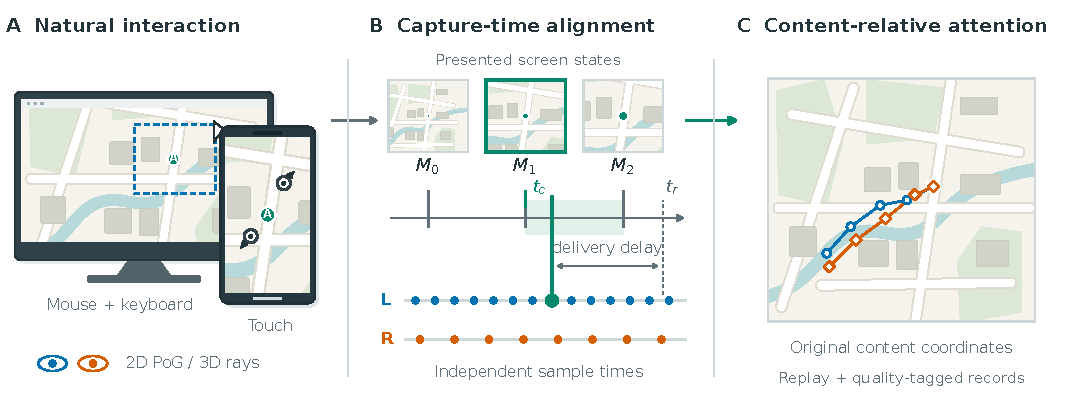
\includegraphics[width=\textwidth]{architecture.pdf}
\caption{GazeSync separates screen presentation and eye-tracking acquisition until capture-time reconstruction. Input commands describe intent; the host records the view actually rendered. Each eye retains its timestamp, coordinate convention and validity. The same recording contract drives Python and TypeScript.}
\Description{Two independent streams, screen interaction and eye observations, feed presentation history and source-clock mapping. Both enter capture-time reconstruction, yielding content-relative attention, raw records, diagnostics and replay.}
\label{fig:architecture}
\end{teaserfigure}
\maketitle

\section{Introduction}
A person zooms into a map landmark, drags the map, and then resets the view. A
screen-coordinate gaze point can refer to three different content locations
during that sequence. A delayed tracker callback adds another ambiguity: the
view visible when the callback is handled may differ from the view at exposure.
On a phone, simultaneous finger movement and changing display pose introduce
further spatial dependencies. Researchers need to distinguish these effects
before interpreting a trace as attention to a particular feature.

The original GazeSync introduced mobile gaze and image-transform logging with
content-relative reconstruction~\cite{gazesync}. This report extends that
system's implementation boundary. It defines how a renderer and heterogeneous
gaze sources exchange timing, geometry and validity, then provides matching
Python and TypeScript implementations. The target is instrumentation of an
application owned by the researcher: the library does not observe arbitrary
operating-system windows or infer unrecorded visual states.

Our contribution has three parts. First, a capture-time contract preserves the
screen state and source provenance needed to reconstruct content-relative gaze.
Second, independent eye channels, source adapters and actionable diagnostics
make heterogeneous measurements explicit. Third, deterministic simulations,
cross-language conformance and isolated distribution artifacts make the
implementation inspectable and repeatable. The evidence is a software audit and
synthetic validation; no new participant or physical-device study is claimed.
The development repository is \url{https://github.com/GazeLei/GazeSync}.

\section{Background and scope}
\subsection{Relationship to the original GazeSync}
The prior system used a Flutter/iOS application with an on-device gaze SDK and
local logging server. Its callback pairing and nearest-state merge used a
50\,ms tolerance. A three-participant formative study illustrated both useful
content-relative reconstruction and calibration or compound-transform
limitations~\cite{gazesync}. Those participants and outcomes belong to the prior
paper; they are not additional validation of this implementation.

The extension replaces the platform-specific merging assumption with explicit
presentation intervals, source clocks and quality decisions. It adds desktop
interaction, independent eye identity, metric ray projection, reusable adapters
and a common record format across languages. Table~\ref{tab:scope} states the
boundary between capabilities and evidence. A source can be accepted at many
frequencies without establishing that a particular device exposes accurate
capture timestamps at those frequencies.

\begin{table}[t]
\caption{Implemented scope and evidence. ``Supported'' denotes a software contract, not certification of a device or browser.}
\label{tab:scope}\small
\begin{tabularx}{\columnwidth}{@{}p{.24\columnwidth}Y@{}}
\toprule
Layer & Capability and evidence \\
\midrule
Interaction & Desktop and mobile controller; deterministic gesture regressions and browser adapter tests. \\
Measurements & 2D PoG, 3D rays, direction-only records; independent and combined eyes with synthetic fixtures. \\
Acquisition & Model and tracker record normalizers; SDKs, transports and physical calibration supplied by the host. \\
Synchronization & Clock mapping, presentation history and uncertainty flags; known-clock synthetic experiments. \\
Distribution & Python wheel/sdist and typed npm package; local installation checks, publication disabled. \\
\bottomrule
\end{tabularx}
\end{table}

\subsection{Interaction and synchronization systems}
Gaze-supported pan and zoom has been investigated as an interaction technique,
including combining gaze with other input modalities~\cite{stellmach}. Our
instrumentation observes manual interaction while retaining gaze for analysis;
it does not assume that the gaze target is the pointer or pinch midpoint. A
person may inspect a landmark while it moves, look at a stable screen location
while dragging, or shift attention ahead of the next action. The simulation
therefore exercises several attention policies instead of coupling the gaze
position directly to the input device.

Lab Streaming Layer provides timestamped multimodal streams and network clock
synchronization~\cite{lsl}. Such infrastructure can supply a transport or clock
estimate to a GazeSync host. Our core instead specifies which rendered content
state a mapped timestamp refers to, how coordinates are reconstructed, and what
makes the result ambiguous. It neither implements a network clock estimator nor
claims to replace multimodal acquisition infrastructure. Device-specific data
contracts also remain consequential: Tobii display coordinates and metric user
coordinates differ from Pupil scene-camera coordinates~\cite{tobii,pupil}.
Explicit normalization is therefore part of the measurement contract, not a
cosmetic import step.

\section{Design requirements}
\paragraph{Record what changed on screen.}
Mouse, keyboard and touch events express intent. A renderer can coalesce many
inputs into one display update or animate a single command across several
frames. We record input events for explanation and presentation snapshots for
reconstruction. A snapshot includes surface, layout epoch, content identity,
viewport dimensions, the rendered affine matrix, timing provenance and optional
registered display geometry. Layout changes and suspension are observable events.

\paragraph{Respect independent measurements.}
A binocular tracker can lose one eye, sample eyes at different times, or expose a
fused output with different semantics. The record retains \code{left},
\code{right}, \code{combined} or \code{unknown} identity. Separate observations
retain their timestamps and validity. The software does not synthesize a second
eye from a combined estimate or treat vendor validity as a probability.

\paragraph{Keep disagreement visible.}
Missing history, uncertain clocks, incompatible coordinates and invalid samples
must remain inspectable. A seemingly smooth trace can conceal an acquisition
error. Raw data and quality flags are retained alongside derived coordinates;
blinks and gaps break a plotted trace. Rates and thresholds are configurable
study parameters rather than universal recommendations.

\paragraph{Keep adaptation local and testable.}
The synchronization core depends on neither a hardware SDK nor a learned model.
Adapters convert explicit records at the edge, while a single finite-JSON
contract carries the result. This permits hardware or inference changes without
changing the content-reconstruction rules. Cross-language fixtures check that
Python analysis and TypeScript acquisition interpret the same record consistently.

\section{Temporal reconstruction}
\subsection{Four event times and a clock epoch}
We distinguish input time $t_i$, presentation time $t_p$, source capture time
$t_s$ and session receipt time $t_r$. A frozen mapping for clock epoch $e$ converts
source time to session capture time:
\begin{equation}
 t_c=b_e+r_e(t_s-a_e),
 \label{eq:clock}
\end{equation}
where $a_e$ and $b_e$ are corresponding anchors and $r_e$ is the clock-rate ratio.
Canonical times are monotonic milliseconds. Browser timing follows the monotonic
clock model of High Resolution Time~\cite{hrtime}; an epoch wall clock cannot be
substituted without a measured mapping.

The host supplies clock uncertainty and optional drift uncertainty. The latter
grows with distance from the anchor; conversion also includes a conservative
floating-point term. A revised fit or source restart requires a new epoch.
These are supplied engineering bounds, not a fitted statistical confidence
interval. The framework does not estimate clock parameters from network arrival
or assume symmetric one-way transport delay. Receipt-only sources remain
recordable but are excluded from capture-time attention analysis.

\subsection{Presentation intervals and ordering}
For the surface-specific history $\mathcal H_s$, alignment selects
\begin{equation}
 j^*=\operatorname*{arg\,max}_{j\in\mathcal H_s:\,t^p_j\leq t_c}
       (t^p_j,\mathrm{sequence}_j).
 \label{eq:selection}
\end{equation}
The last submitted snapshot wins a timestamp tie. Each snapshot persists until
its successor. Geometry is not interpolated through an unobserved animation,
reset or content replacement. The host must record every relevant intermediate
rendered state, or explicitly assert change-only presentation logging.

A call to \code{flush(h)} is a watermark: it declares that all presentations
through $h$ have already been submitted. Insertion at or before that watermark
is rejected. Samples normally wait for the greater of the configured reorder
window and maximum accepted clock uncertainty. Ready samples are sorted by
capture time within each flush. Later arrivals remain identifiable even when
retained history permits valid offline reconstruction. Impossible future times
and excessive uncertainty are quarantined promptly, preventing indefinite
pending-buffer growth.

The interval $[t_c-u_c,t_c+u_c]$ is checked against visual changes. If it crosses a
relevant change, the output is marked ambiguous. Boundaries that repeat identical
geometry do not create false ambiguity. Histories are indexed per surface;
retention preserves the newest state of each active surface, so frequent updates
on one display do not evict another display's only state. A required older state
may still expire, producing an explicit history flag.

\begin{figure*}[t]
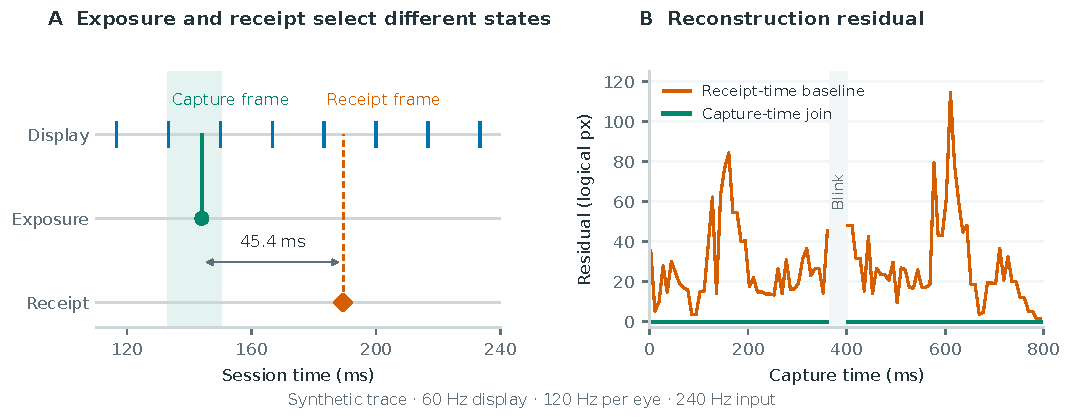
\includegraphics[width=\textwidth]{timing.pdf}
\caption{A representative synthetic trace at 60\,Hz display, 240\,Hz input and 120\,Hz gaze per eye. (A) The same sample selects different display intervals at exposure and receipt. The shaded interval contains the true capture time. (B) Using receipt time produces content-reconstruction error during view change; capture-time residuals remain at numerical scale. The blink interval is missing data. Both panels are generated from saved simulation outputs, not a physical timing measurement.}
\Description{Left: presentation ticks, one exposure and its later receipt, with different selected intervals. Right: an orange receipt-time residual varies over 800 milliseconds, whereas the green capture-time residual lies near zero. A blink interval is shaded.}
\label{fig:timing}
\end{figure*}

\subsection{Why timing errors become spatial errors}
For a viewport observation $p_v$ and rendered matrix $M(t)$, content gaze is
$M(t)^{-1}\widetilde p_v$. Away from discontinuities, a small timing displacement
$\Delta t$ yields a first-order spatial error proportional to
\begin{equation}
 \left\|\frac{d M(t)^{-1}}{dt}\widetilde p_v\right\|\,|\Delta t|.
\end{equation}
Fast zoom or translation can therefore amplify a modest delivery delay. At a
reset or layout discontinuity this derivative approximation does not apply;
the correct presentation interval must be selected explicitly.
Figure~\ref{fig:timing} illustrates this mechanism with known synthetic timing.
The receipt-time baseline is an intentionally incorrect association policy,
not a benchmark against every strategy used by existing systems.

\section{Spatial reconstruction and eye identity}
\subsection{Two-dimensional points and content transforms}
A PoG declares viewport, normalized-viewport or normalized-display coordinates.
The full-display case requires recorded display dimensions and viewport offsets
in compatible units. Device pixel ratio is retained as metadata and is not an
instruction to multiply logical coordinates again. The renderer supplies
\begin{equation}
 M=\begin{bmatrix}a&c&e\\b&d&f\\0&0&1\end{bmatrix},
 \qquad \widetilde p_c=M^{-1}\widetilde p_v.
\end{equation}
This representation includes letterboxing, intrinsic image scaling, pivot
translation and rotation without applying an offset twice. Coordinates outside
the viewport or content remain visible and flagged rather than being clipped
to an apparently valid target.

Each accepted frame caches its inverse. The inversion checks conditioning after
normalizing the linear block by its largest absolute coefficient. It rejects
singular or non-finite results while permitting uniformly small, well-conditioned
transforms. This matters for large content coordinate systems whose displayed
scale can be much less than one.

\subsection{Metric rays and a registered display}
A ray supplies origin $O$ in metres, direction $D$ and a frame identifier. The
registered display supplies top-left point $P$, orthonormal right/down axes
$u,v$ and metric dimensions $w_m,h_m$. After normalizing $D$, the forward crossing is
\begin{equation}
 n=u\times v,\quad
 \lambda=\frac{(P-O)\cdot n}{D\cdot n},\quad
 Q=O+\lambda D.
\end{equation}
Zero, nearly parallel, backwards or incompatible rays do not fabricate a hit.
For viewport size $W\times H$,
\begin{equation}
 p_v=\left(W\frac{(Q-P)\cdot u}{w_m},\;
           H\frac{(Q-P)\cdot v}{h_m}\right).
\end{equation}
The same content inverse then applies. This is a crossing of a registered display
plane, not an inferred scene fixation or vergence depth.

Moving displays require pose timestamps and measured extrinsics. The current
implementation uses the selected frame's recorded pose and checks its age; it
does not interpolate unobserved sub-frame motion. A direction-only model output
is retained as \code{direction3d} but cannot be projected by inventing an eye
origin. Figure~\ref{fig:geometry} makes these dependencies explicit.

\begin{figure}[t]
\centering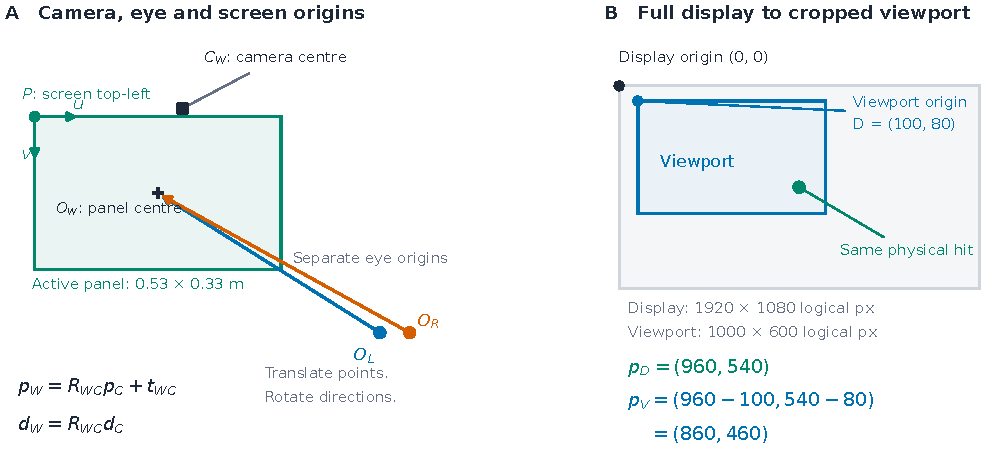
\includegraphics[width=.98\columnwidth]{geometry.pdf}
\caption{Independent eyes retain separate origins, rays, timestamps and validity. The display plane and both rays must share a measured coordinate frame. A schematic 600/120\,Hz timeline illustrates unequal acquisition; optional bounded pairing neither resamples nor averages the eyes. Geometry is illustrative and not to scale.}
\Description{Blue and orange rays start at separate left and right eye origins and intersect a green registered display plane at separate points. Below, two rows show unequal sampling cadence.}
\label{fig:geometry}
\end{figure}

\subsection{Observation identity and optional pairing}
Observation identity includes source, clock ID and epoch, eye, representation
and sample ID. The same physical capture can thus carry left/right and PoG/ray
records without collision. Optional capture and calibration identifiers retain
further provenance. A combined estimate stays combined; no post hoc label turns
it into an independent monocular observation.

For analyses that need matched eyes, an offline helper performs chronological,
one-to-one pairing under a caller-specified maximum skew, defaulting to 5\,ms.
It considers only usable observations with matching source, representation,
clock identity/epoch, surface/epoch and calibration. Unmatched observations are
returned explicitly. Different source clocks can be synchronized by the host,
but the helper conservatively leaves them separate. It does not implement an
optimal assignment, estimate vergence or fuse measurements. Study-specific
fusion requires its own uncertainty and validity policy.

\section{Adapters, diagnostics and developer contract}
\subsection{SDK-independent normalization}
Both language implementations expose generic model, Tobii Pro dictionary,
EyeLink bridge and Pupil Core adapters. A generic model adapter supports nested
field paths, explicit timestamp units, display-pixel normalization and metric
origin conversion. Model inference and tensor transfer remain outside the core.
A new adapter can be a pure function producing the shared JSON schema and
structured warnings.

Tobii normalization preserves per-eye validity and normalized display points;
optional rays are defined from the vendor origin to the reported display point,
with millimetres converted to metres~\cite{tobii}. Confidence remains null when
only validity is provided. The EyeLink bridge consumes serialized per-eye pixel
records and millisecond device timestamps; a Python helper extracts this bridge
record from a newly received PyLink sample~\cite{eyelink}. Neither path bundles or
licenses the hardware SDK on the user's behalf.

Pupil normalization preserves individual base-sample timestamps and deduplicates
reused eye observations within a bounded history. Scene-camera coordinates do
not become screen PoG without an explicit calibrated homography or registered
surface record. Right/left IDs, bottom-origin coordinates and millimetre eye
centres follow the vendor contract~\cite{pupil}. Mapping timestamp skew is
retained and checked. These behaviors are tested with synthetic protocol
fixtures; the release does not claim physical tracker validation.

\subsection{Diagnostics as integration feedback}
A source descriptor declares adapter, eye set, tracking mode, expected cadence
and timestamp provenance. Expected cadence does not resample observations.
Diagnostics estimate rates per source, eye, representation and clock epoch
using bounded windows. They expose gaps, out-of-order delivery, rate deviations,
missing history, uncertain clocks and unavailable geometry. Observers receive
the first occurrence for each diagnostic context while the report retains counts
and most recent occurrence times. An observer exception is recorded without
interrupting acquisition.

A per-observation \code{usable} flag and reason list remain the primary quality
contract. Informational conditions, such as unavailable scalar confidence, can
coexist with usable geometry. Receipt-only timestamps, blinks, missing history
or ambiguous presentation make content attention unusable. Raw measurements
remain available for a different downstream analysis that states its own policy.

\subsection{Human interaction and host responsibilities}
The controller anchors wheel zoom at the pointer, distinguishes drag from
selection-box zoom, supports keyboard reset and cancels an active gesture when
another view command takes over. Touch interaction tracks contacts, pinch scale
and midpoint translation; releasing one contact transitions to pan without a
jump. Double tap, cancellation, resize, orientation change and background/resume
are explicit cases. Browser handling follows pointer-event ownership and
cancellation semantics~\cite{pointerevents}; it avoids capturing keys from
embedded editable controls.

The browser adapter records application input, while the host records what was
rendered. Native Python applications can feed the same controller logic from
GUI callbacks. Both cores are synchronous; applications serialize rendering and
SDK callbacks through a single session owner. No transport or thread scheduler
is hidden in the measurement path. Host-specific kinetic scrolling or animation
can be recorded as presentation snapshots without adding its physics to the core.

\section{Verification and synthetic evaluation}
\subsection{Audit strategy and regression coverage}
The audit follows failure paths across geometry, event ordering, browser input,
recording, replay and package boundaries. Earlier defects included cross-surface
frame selection, keyboard zoom overwritten by a stale drag baseline, unstable
small-scale inversion, malformed-record mutation, delayed future-time quarantine
and undetected replay gaps. Focused regression tests reproduce those triggers.
The extension adds explicit eye identity, shared adapter fixtures, receipt-time
exclusion, nullable confidence and clock-boundary checks in both languages.

Strict TypeScript compilation generates public declarations from the executable
source. Consumer tests check exports and validity-dependent measurement types.
Python tests exercise the independent implementation and validate normalized
fixtures against JSON Schema. Release checks inspect imports, package contents,
license consistency and shared fixtures. These tests establish specified
behaviors under examined inputs; they are not a proof of general correctness.

\subsection{Two complementary simulation families}
\paragraph{Interaction scenarios.}
Desktop and mobile scenarios each last nine seconds at 60\,Hz display and
120\,Hz gaze, repeated with seeds 1, 41 and 90210. Desktop actions include wheel
zoom, pan, marquee selection, cancellation, reset and resize. Mobile actions
include pinch in/out, moving midpoint, pinch-to-pan transition, double tap,
orientation and suspension. Attention policies include content-landmark tracking,
screen-fixed attention during pan, scanning and reading-like fixation steps.
Timing and motion parameters are illustrative test assumptions, not a fitted
model of human eye movements. The moving-phone fixture holds pose between
recorded frames and does not validate real continuous motion.

\paragraph{Rate and context matrix.}
A second family separates frequency sensitivity from context coverage. The
controlled matrix contains 42 cells: six display rates (30, 60, 90, 120, 144 and
240\,Hz) crossed with seven gaze rates per eye (30, 60, 120, 250, 600, 1,000 and
2,000\,Hz). It fixes a $1280\times720$ viewport, 240\,Hz input and independent
binocular acquisition. A further 36 cases cross nine viewport configurations
with left monocular, right monocular, independent binocular and combined modes.
These context cases vary input rate, device pixel ratio, orientation and clock
configuration together; they are coverage cases, not a factorial causal study.

The nine initial viewports range from $320\times568$ to $3840\times2160$, including
portrait, landscape, tablet and ultrawide layouts. Context input rates range
from 30 to 1,000\,Hz. Independent context eyes use 600 and 120\,Hz and separate
clock mappings. Each case lasts 800\,ms with seed 41. Inputs are coalesced into
rendered frames. Ordinary delivery delay is 28--63\,ms, with an additional
120\,ms on selected captures. A blink interval occupies 46--50\% of the trace.
Uniform per-axis perturbation of $\pm0.35$ logical pixels supplies an explicitly
high-accuracy synthetic source; it is not a camera-model accuracy estimate.

PoG and ray observations originate from the same perturbed viewport target.
Their agreement tests representation consistency rather than agreement between
independent sensors. Reconstruction error is measured against that perturbed
target, using the known renderer coefficients, and expressed back in logical
viewport pixels. Sensor noise is therefore distinguished from software
reconstruction residual. No human data are used in either simulation family.

\begin{figure*}[t]
\centering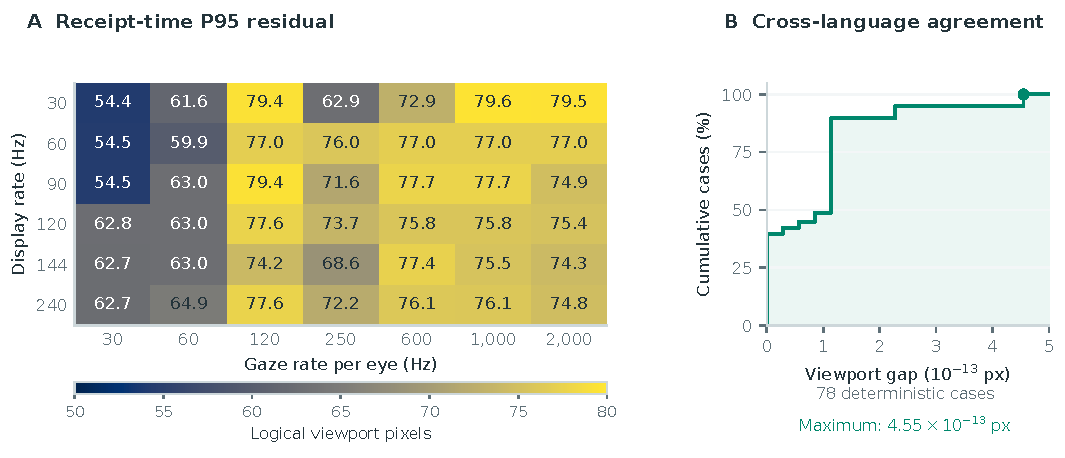
\includegraphics[width=\textwidth]{validation.pdf}
\caption{Controlled rate experiment and overall software checks. (A) P95 residual when deliberately using the receipt-time frame, at fixed $1280\times720$, 240\,Hz input and independent binocular gaze; each cell is one seeded 800\,ms trace. Values are descriptive, without participant-level inference. (B) The 42 rate cells and 36 additional context cases yield 107,070 observations. Correct capture-time reconstruction has zero frame mismatches and numerical-scale residuals. The extra context cases are reported separately because viewport, rate and orientation vary together.}
\Description{A six-by-seven heatmap reports receipt-time baseline error by display and gaze frequency. A separate panel lists 78 configurations, 107070 observations and zero frame mismatches, with a maximum numerical reconstruction residual of 7.85 times ten to the minus thirteen logical pixels.}
\label{fig:validation}
\end{figure*}

\subsection{Cross-language conformance and results}
The test driver serializes identical events for both implementations and compares
all aligned records and diagnostic reports. Keys, labels, frame identities and
flags must match exactly. Numeric comparison uses absolute tolerance $10^{-8}$
plus relative tolerance $10^{-12}$; the largest observed differences are much
smaller (Table~\ref{tab:results}). The suite additionally compares ten source
adapter fixtures and checks exact replay of derived alignment within the same
implementation. Python-native experiment generation is exercised separately.

Across the 78 cases, all 107,070 expected observations are received, pending
buffers drain, and every capture-frame selection matches the independent
synthetic reference. Maximum reconstruction residual is
$7.85\times10^{-13}$ logical pixels. Maximum Python--TypeScript viewport
disagreement is $4.55\times10^{-13}$ pixels; mapped capture times agree at the
reported precision. These near-zero values measure arithmetic and contract
consistency for known inputs. They cannot establish subpixel physical accuracy.

The receipt-time baseline's P95 residual ranges from 54.4 to 79.6 logical pixels
across the controlled cells (Figure~\ref{fig:validation}A). This range belongs to
the specified fast manipulation trace, viewport and delays. It is not a general
error bound or a comparison between tracker brands. Increasing gaze rate cannot
repair an incorrect temporal association. Context-case baseline values are not
pooled to infer frequency effects because dimensions and motions also differ.

\begin{table}[t]
\caption{Numerical consistency on the 78-case matrix. Units distinguish content coordinates from logical viewport pixels.}
\label{tab:results}\small
\begin{tabularx}{\columnwidth}{@{}Yr@{}}
\toprule
Measure & Observed result \\
\midrule
Expected / received observations & 107,070 / 107,070 \\
Capture-frame mismatches & 0 \\
Maximum reconstruction residual (px) & $7.85\times10^{-13}$ \\
Maximum cross-language viewport difference (px) & $4.55\times10^{-13}$ \\
Maximum cross-language content difference (units) & $4.55\times10^{-13}$ \\
Maximum capture-time difference (ms) & 0 \\
Exact within-implementation replay & 78 / 78 cases \\
Pending observations after final drain & 0 \\
\bottomrule
\end{tabularx}
\end{table}

\section{Reproducibility and distribution}
The repository contains strict TypeScript source, Python source, JSON schemas,
synthetic fixtures, regression tests, a local interaction lab and figure scripts.
The two libraries have no runtime dependencies. npm ships executable modules,
generated declarations and corresponding TypeScript source. Python ships a wheel
and source distribution; SDKs, inference weights and private-project data are
excluded. Clean installation tests run outside the checkout, including a wheel
rebuilt from the source distribution.

Schema 2.0 records the implementation version, source descriptors, clock
mappings, configuration, raw event sequence, retention losses and derived output.
Exact replay rejects incomplete or incompatible logs. Default in-memory limits
are explicit: 7,200 frames, 100,000 raw/derived records and 4,096 pending
observations. Long sessions require persistence before rollover. Current bounded
arrays still incur front-removal costs; streaming storage and backpressure
remain measured integration work rather than claimed features.

The full matrix can be reproduced with the following source-checkout commands:
\begin{lstlisting}
npm run test:conformance
node tools/paper-data.mjs
.venv/bin/python tools/paper_figures.py
\end{lstlisting}
Figure generation additionally requires the pinned plotting dependencies listed
in the paper build guide. The reported local run used Node.js 26.7.0 and Python
3.12.14. Continuous integration is configured across Node 22/24/26 and Python
3.10/3.12/3.14. The aggregate JSON data preserve every configuration and result;
generated working sessions remain excluded from source control.

Code is licensed GPL-3.0-only. The manuscript has separate draft publication
rights. The repository is currently private and registry publishing is disabled;
no public package availability or implementation arXiv identifier is claimed.
Maintainer-reviewed workflows prepare the official npm and PyPI routes. Citation
metadata requests both the original GazeSync paper and this implementation report;
it will be updated with the real preprint identifier after submission.

\section{Limitations and evaluation agenda}
The largest uncertainty lies outside the synthetic equations: physical exposure
time, display scanout, clock offset and drift, extrinsic calibration, source
accuracy and moving-device pose. Render callbacks alone do not measure photon
onset. Replaying known geometry cannot validate an assumed camera-to-display
transform. Protocol fixtures cannot establish behavior across firmware or SDK
versions, and a phone-sized browser simulation cannot certify touch behavior on
every mobile browser.

The next evaluation should measure timing against an external reference, report
latency distributions and uncertainty, and test display geometry on held-out
targets. Static views, pan, zoom, rotation and device motion should be assessed
separately before compound manipulations. Relevant outcomes include temporal
ambiguity, usable coverage, per-eye dropout, viewport/content error and angular
ray error. Calibration and assessment targets must remain separate. Repeated
sessions and participant-separated analysis are needed to characterize drift
and generalization.

Human behavior also needs empirical grounding. The scripted attention policies
exercise distinct reconstruction cases but do not estimate how often people
follow a pointer, retain a landmark or look ahead of an action. A future study
should record task intent and interaction phases alongside independent gaze,
then test whether the instrumentation preserves meaningful content attention
without changing normal interaction. Longer runs should measure memory,
persistence overhead and worst-case latency under realistic acquisition load.

\section{Conclusion}
GazeSync provides an explicit bridge between heterogeneous eye-tracking records
and the content state visible during desktop or mobile interaction. Its temporal
contract, geometric conventions, independent eye records and quality flags make
assumptions inspectable. Matching Python and TypeScript implementations, adapter
fixtures and synthetic experiments establish a reproducible software foundation.
Measured device timing, calibration and participant behavior remain the necessary
next evidence for end-to-end claims.

\begin{thebibliography}{9}
\bibitem{gazesync} Yaxiong Lei, Rishab Talwar, Shijing He, Xinya Gong, Yuheng Wang, Xudong Cai, Zhongliang Guo, and Juan Ye. 2026. GazeSync: A Mobile Eye-Tracking Tool for Analyzing Visual Attention on Dynamically Manipulated Content. In \textit{Extended Abstracts of the CHI Conference on Human Factors in Computing Systems}. \url{https://doi.org/10.1145/3772363.3798725}
\bibitem{stellmach} Sophie Stellmach and Raimund Dachselt. 2012. Investigating Gaze-supported Multimodal Pan and Zoom. In \textit{Proceedings of the Symposium on Eye Tracking Research and Applications (ETRA)}. \url{https://imld.de/cnt/uploads/2013/07/2012-ETRA-GazeSuppPanAndZoom.pdf}
\bibitem{lsl} Christian Kothe, Seyed Yahya Shirazi, Tristan Stenner, David Medine, Chadwick Boulay, Matthew I. Grivich, Fiorenzo Artoni, Tim Mullen, Arnaud Delorme, and Scott Makeig. 2025. The lab streaming layer for synchronized multimodal recording. \textit{Imaging Neuroscience} 3. \url{https://doi.org/10.1162/IMAG.a.136}
\bibitem{tobii} Tobii Pro. Coordinate systems and Python SDK documentation. \url{https://developer.tobiipro.com/commonconcepts/coordinatesystems.html}. Accessed 15 October 2026.
\bibitem{pupil} Pupil Labs. Pupil Core developer documentation. \url{https://docs.pupil-labs.com/core/developer/}. Accessed 15 October 2026.
\bibitem{eyelink} SR Research. Python programming with EyeLink. \url{https://www.sr-research.com/support/thread-48-post-47.html}. Accessed 15 October 2026.
\bibitem{hrtime} W3C. High Resolution Time, Level 3. \url{https://www.w3.org/TR/hr-time-3/}. Accessed 15 October 2026.
\bibitem{pointerevents} W3C. Pointer Events, Level 3. \url{https://www.w3.org/TR/pointerevents3/}. Accessed 15 October 2026.
\end{thebibliography}
\end{document}
